\clearpage
\section*{二、实验操作与原始数据}

\subsection*{1. 实验操作与原始记录}

实验在 1 号桌进行。我先调平测量室，喷入油滴后调节显微镜焦距，在显示屏上挑选油滴；随后把 K2 依次拨到“平衡”“提升”“0V”挡，记录平衡电压 $U$ 和油滴匀速下落 $l=1.5\,\mathrm{mm}$ 所用的时间 $t$。按本次要求，共测 5 个油滴，每个油滴测量两次。

数据由 Omwin 密立根油滴实验数据处理程序（Ver1.6）记录和计算，参数设置见下图。其中空气黏滞系数取 $1.83\times10^{-5}\,\mathrm{N\cdot s/m^2}$，比教材的 $1.82\times10^{-5}$ 略大，其余参数与教材一致。

\begin{figure}[H]\centering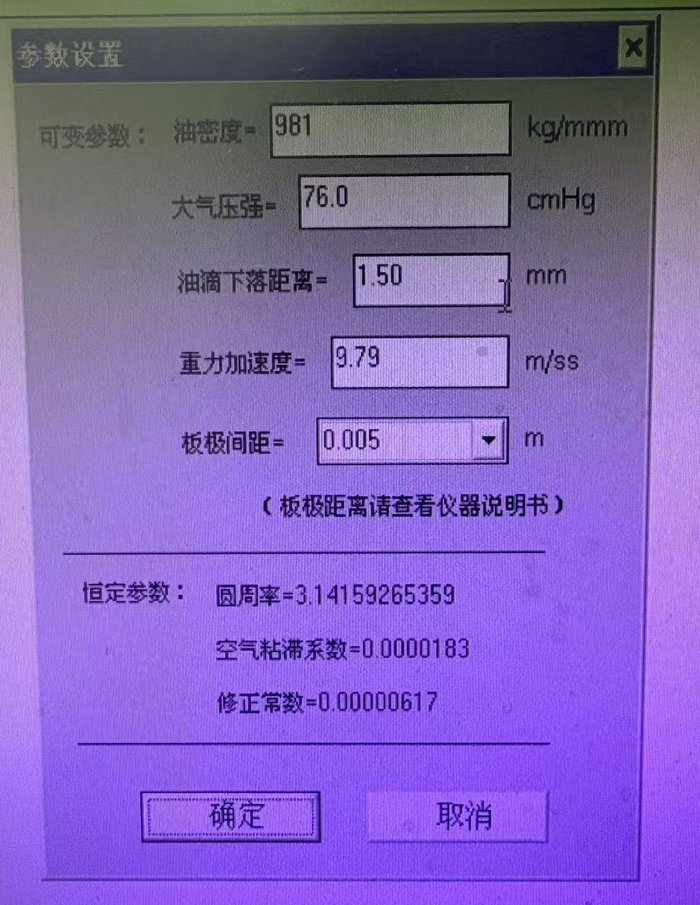
\includegraphics[width=5.6cm]{../assets/software-params.jpg}\caption{数据处理软件的参数设置}\end{figure}

原始记录如下。记录表第四行标为 $q_i$，实际抄录的是软件给出的单个电子电荷值 $e$。

\begin{figure}[H]\centering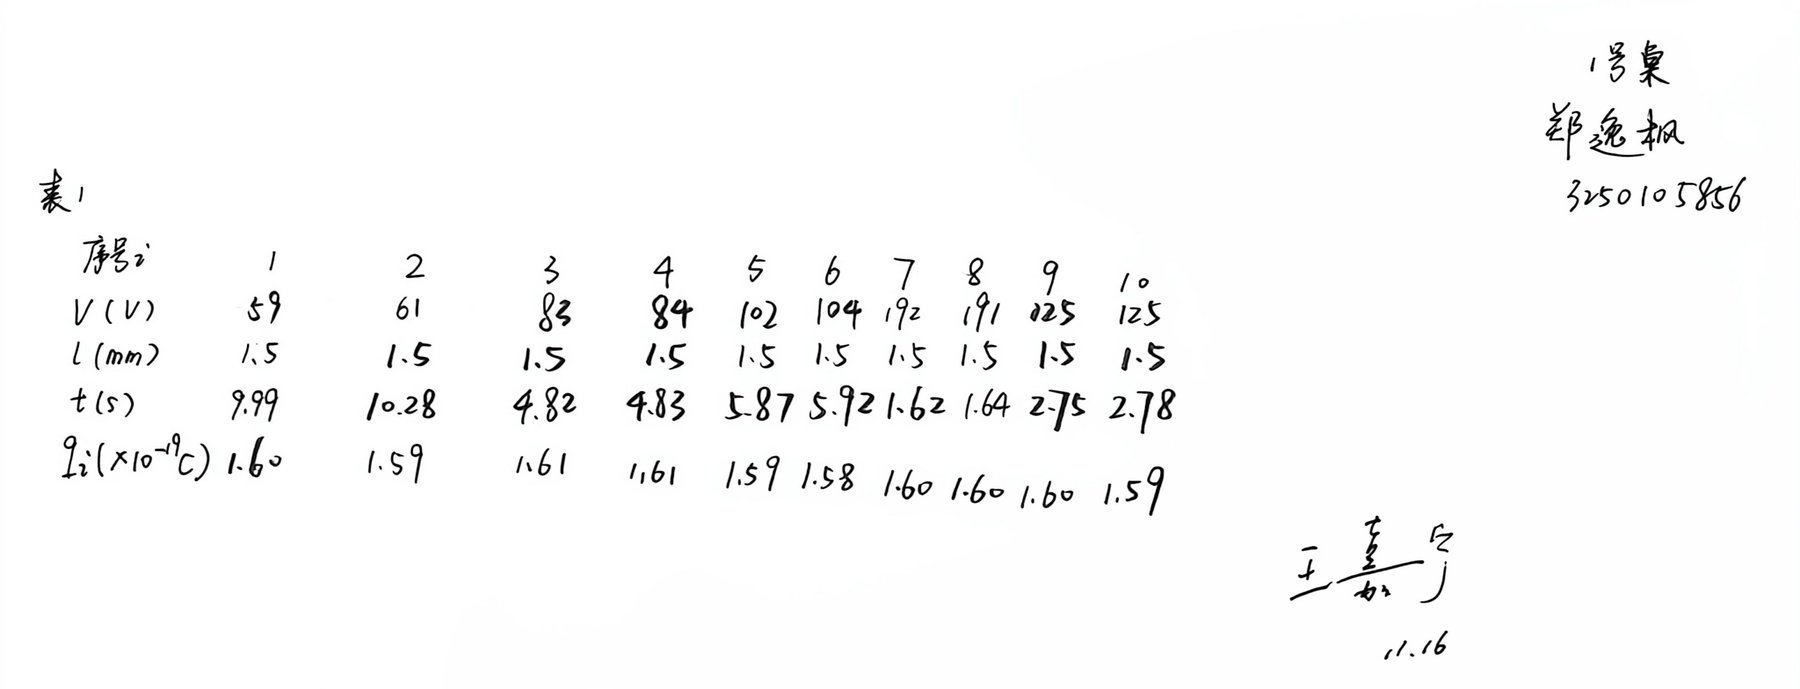
\includegraphics[width=16cm]{../assets/raw-data.jpg}\caption{本次原始记录}\end{figure}

\clearpage

\subsection*{2. 测量数据}

\begin{center}\small\setlength{\tabcolsep}{4pt}
\begin{tabular}{ccccccccccc}
\toprule
序号 $i$ & 1 & 2 & 3 & 4 & 5 & 6 & 7 & 8 & 9 & 10 \\
\midrule
油滴编号 & 1 & 1 & 2 & 2 & 3 & 3 & 4 & 4 & 5 & 5 \\
$U$/V & 59 & 61 & 83 & 84 & 102 & 104 & 192 & 191 & 125 & 125 \\
$l$/mm & 1.5 & 1.5 & 1.5 & 1.5 & 1.5 & 1.5 & 1.5 & 1.5 & 1.5 & 1.5 \\
$t$/s & 9.99 & 10.28 & 4.82 & 4.83 & 5.87 & 5.92 & 1.62 & 1.64 & 2.75 & 2.78 \\
\bottomrule\end{tabular}\end{center}

软件对每次测量给出的电荷值 $q$、电子数 $n$ 和电子电荷值 $e$ 如下。

\begin{center}\small\setlength{\tabcolsep}{4pt}
\begin{tabular}{ccccccccccc}
\toprule
序号 $i$ & 1 & 2 & 3 & 4 & 5 & 6 & 7 & 8 & 9 & 10 \\
\midrule
$q$/(10$^{-19}$ C) & 44.9 & 41.5 & 98.2 & 96.7 & 59.0 & 57.1 & 224 & 221 & 154 & 151 \\
$n$ & 28 & 26 & 61 & 60 & 37 & 36 & 140 & 138 & 96 & 95 \\
$e$/(10$^{-19}$ C) & 1.60 & 1.59 & 1.61 & 1.61 & 1.59 & 1.58 & 1.60 & 1.60 & 1.60 & 1.59 \\
\bottomrule\end{tabular}\end{center}

\subsection*{3. 软件截图}

\begin{figure}[H]\centering
\begin{minipage}[b]{0.31\linewidth}\centering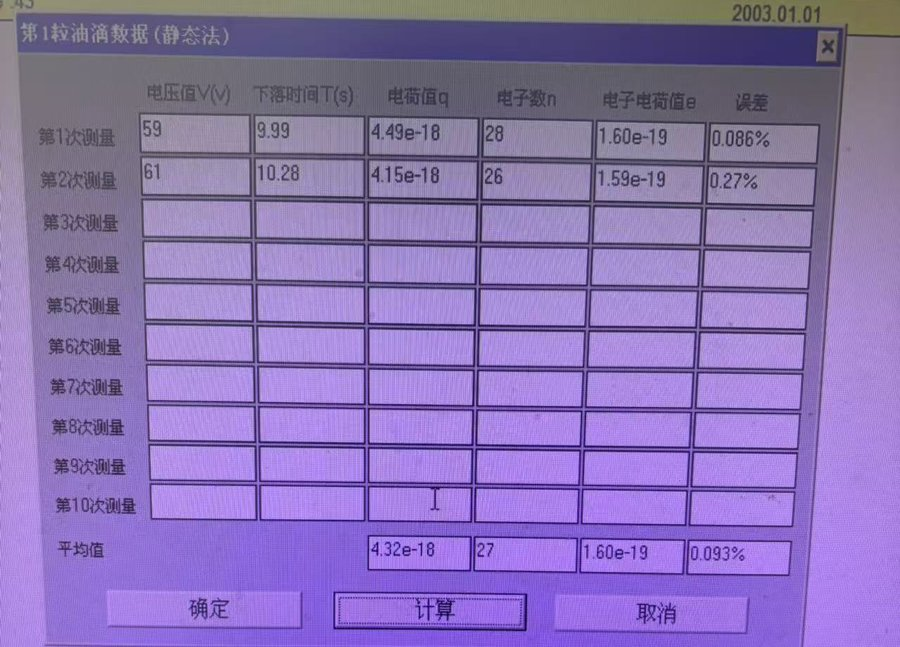
\includegraphics[width=\linewidth]{../assets/software-drop1.jpg}\caption{第 1 粒油滴数据}\end{minipage}\hfill\begin{minipage}[b]{0.31\linewidth}\centering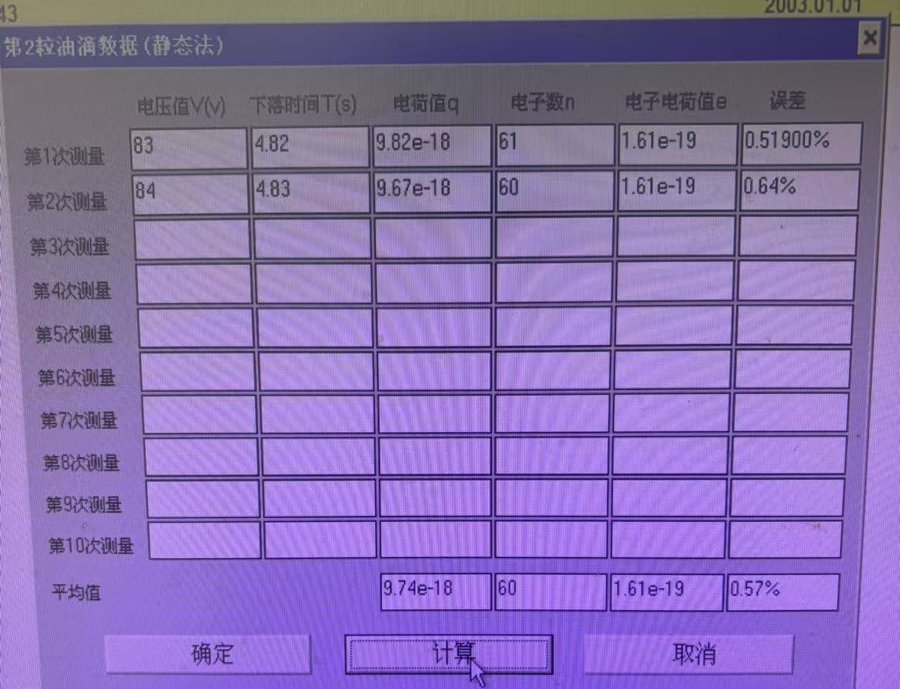
\includegraphics[width=\linewidth]{../assets/software-drop2.jpg}\caption{第 2 粒油滴数据}\end{minipage}\hfill\begin{minipage}[b]{0.31\linewidth}\centering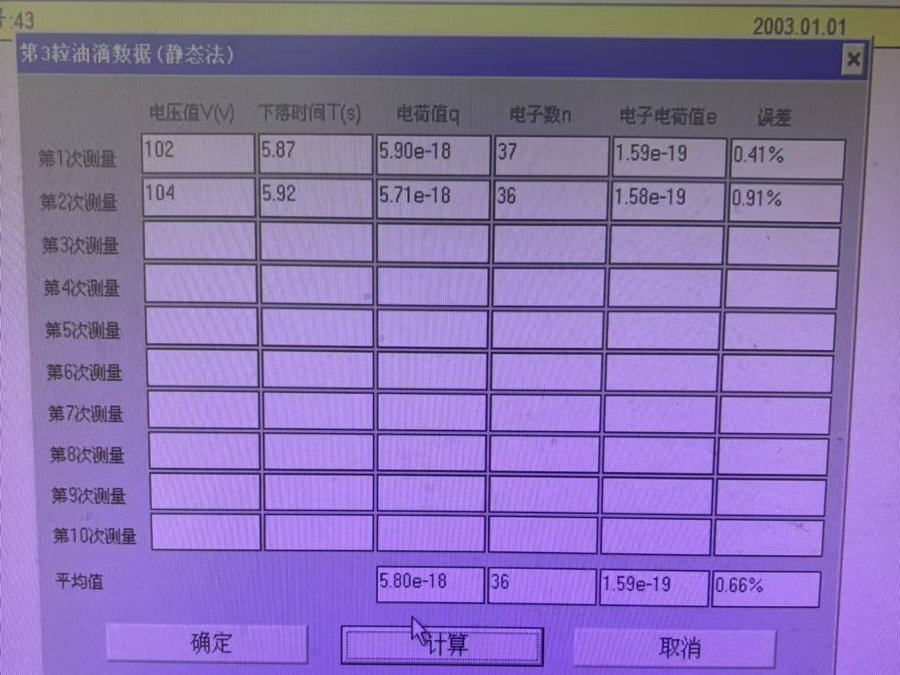
\includegraphics[width=\linewidth]{../assets/software-drop3.jpg}\caption{第 3 粒油滴数据}\end{minipage}
\end{figure}

\begin{figure}[H]\centering
\begin{minipage}[b]{0.31\linewidth}\centering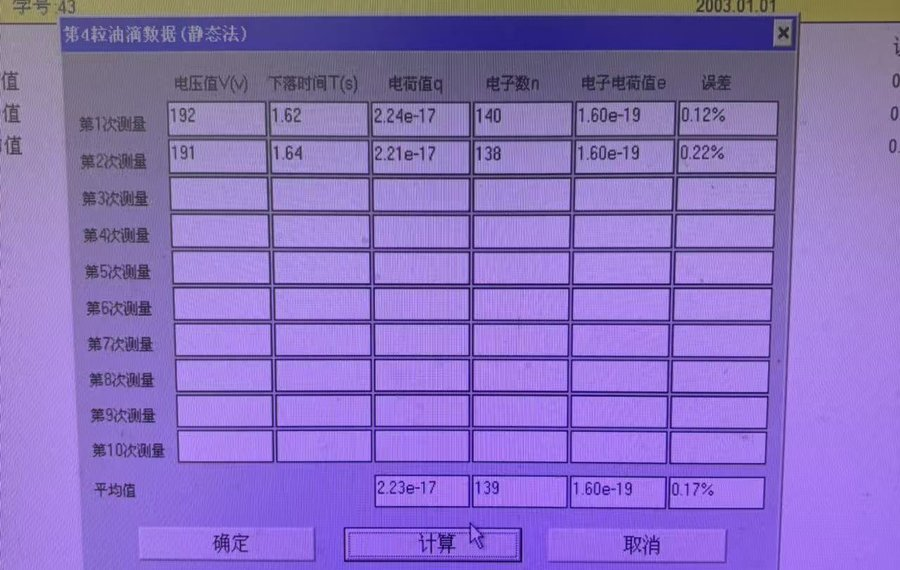
\includegraphics[width=\linewidth]{../assets/software-drop4.jpg}\caption{第 4 粒油滴数据}\end{minipage}\hspace{2em}\begin{minipage}[b]{0.31\linewidth}\centering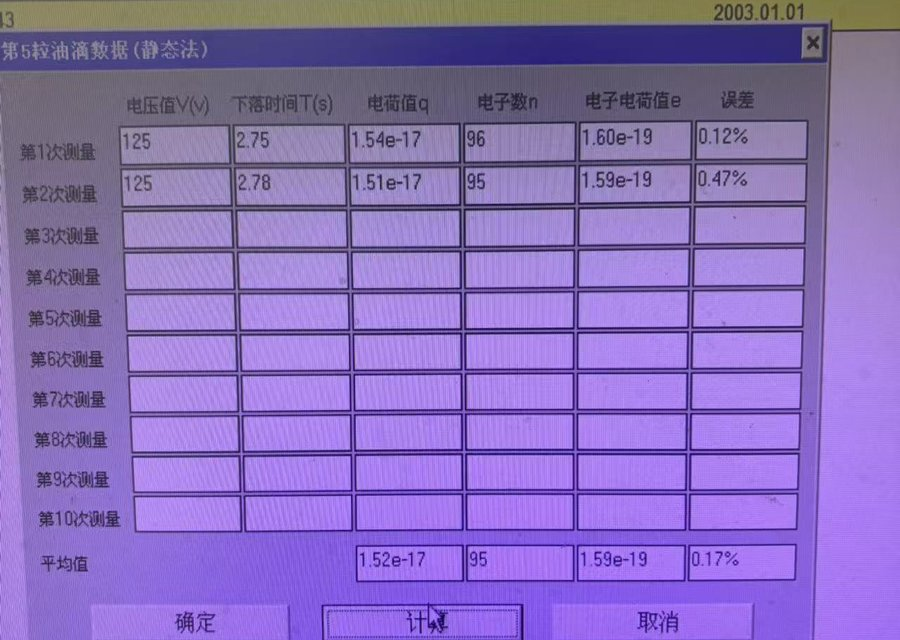
\includegraphics[width=\linewidth]{../assets/software-drop5.jpg}\caption{第 5 粒油滴数据}\end{minipage}
\end{figure}

\begin{figure}[H]\centering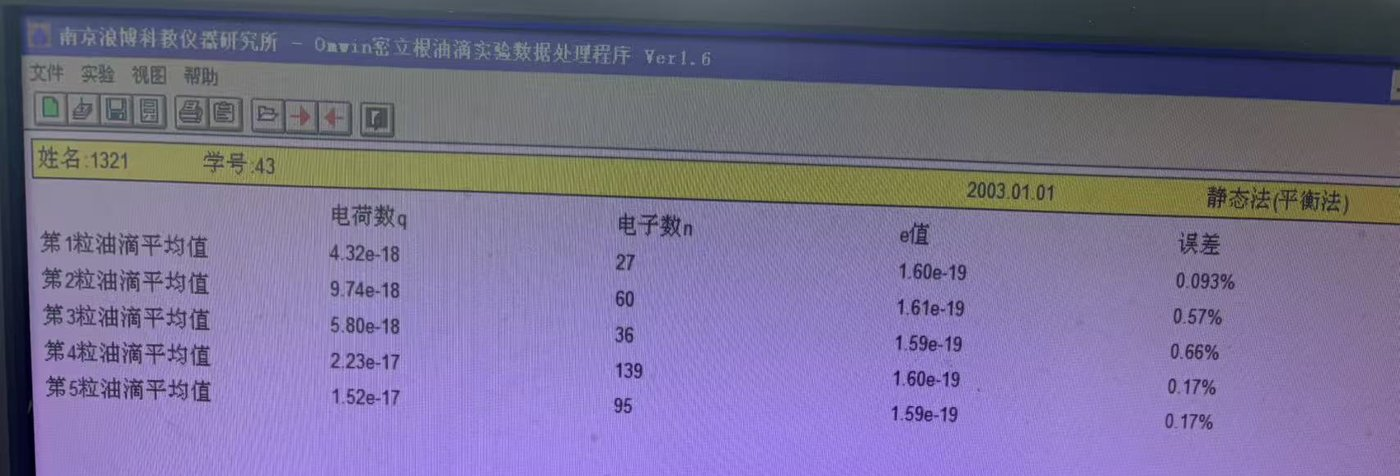
\includegraphics[width=11cm]{../assets/software-summary.jpg}\caption{5 粒油滴平均值总览}\end{figure}

\clearpage

